\documentclass[a4paper,10pt]{article}
\usepackage[english]{babel}
\usepackage{amsmath}
\usepackage{hyperref}
\usepackage{float}
\usepackage{tabularx} 
\usepackage{hhline}
\usepackage{booktabs} 
\usepackage[table]{xcolor}
\usepackage{listings}
%\usepackage{array}
%\usepackage{subfig}
%\usepackage{siunitx}
%\usepackage{color}
%\usepackage{fancyvrb}
\usepackage[pdftex]{graphicx}
\usepackage{fancyhdr}
\pagestyle{fancy}
\usepackage{verbatim}
\fancyhf{}
\cfoot{Version 1}

\newcommand{\HRule}{\rule{\linewidth}{0.5mm}}
\numberwithin{equation}{section}
\numberwithin{figure}{section}
\numberwithin{table}{section}
\parindent=0pt


\begin{document}
	\begin{titlepage}
		
		\begin{center}
			\vspace{15mm}
		\end{center}
		
		\begin{figure}[H]
			\centering
		\end{figure}
		
		\begin{center}
			\vspace{10mm}
			{\Huge Presentatie @Home team Tech United}\\
			\vspace{3mm}
			{\Large Eindhoven University of Technology}\\
			\vspace{10mm}
			\vspace{3mm}
			%\begin{figure}[H]
			%\center
			%\includegraphics[scale=0.6]{AMIGO.jpg}
			%\end{figure}
			\today
		\end{center}
		
		\vfill
		
		
		\begin{tabular}{l l}
			Version 1\\
		\end{tabular}
		
	\end{titlepage}

\section*{Paklijst Demo's}
Met AMIGO kunnen ruwweg 2 verschillende soorten demo's gegeven worden, een interne demo en een externe demo. Voor deze twee verschillende demo's zijn verschillende materialen nodig. De materiaalset voor de interne demo kan gezien worden als een basis set die altijd nodig is, de materialenset voor de externe demo is hier dus een uitbreiding op. Check voor \textbf{ELKE} demo of (op zijn minst) al de benodigde voorwerpen uit de paklijst aanwezig zijn en bedenk of er eventueel extra benodigdheden zijn voor de specifieke demo.

\section{Interne Demo}

\begin{itemize}
	\item \textbf{NOODSTOP}
	\item Demo-tas
	\begin{itemize}
		\item Laptop
		\item Laptop voeding
		\item Router
		\item Netwerkkabel voor router
	\end{itemize}
	\item Batterijen
	\begin{itemize}
		\item Neem 12 losse batterijen mee. Dit geeft dus een totaal van 16 batterijen inclusief de 4 baterijen in de robot
		\item \textbf{Let op!} De batterijen in de robot moeten 1 voor 1 gewisseld worden. Er mag om geen enkele reden meer dan 1 batterij uit de robot zijn.
		\item \textbf{Tip:} Leg de batterijen die leeg zijn op een zijkant  en de batterijen die vol zijn op de achterkant (met de contact punten naar boven gericht), zo is het heel makkelijk te zien welke batterijen vol zijn en welke batterijen niet.
	\end{itemize} 
	\item Tablet
	    \item Demo object set
	    \begin{itemize}
	    	\item Cola blikje 
	    	\item Fanta blikje
	    	\item Ice tea blikje
	    	\item Pringels bus
	    	\item Appel
	    	\item Mandarijn
	    	\item Doosje thee
	    \end{itemize}
	\item Demo shirts
	\item Promotie materiaal
		\begin{itemize}
			\item Stickers
			\item Visite kaartjes
			\item Klompjes
		\end{itemize}
\end{itemize}

\section{Externe Demo}

\begin{itemize}
	\item Audio en media flight-cases
	\item Batterij laders
	\item Stekker batterijen
	\item Meubels
		\begin{itemize}
			\item Hallway table
			
				\begin{figure}[H]
					\centering
					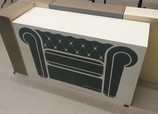
\includegraphics[width=0.3\textwidth]{hallwaytable}
				\end{figure}
			
			\item Couch table
				\begin{figure}[H]
					\centering
					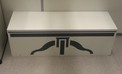
\includegraphics[width=0.3\textwidth]{couchtable}
				\end{figure}			
			
			\item Bar
				\begin{figure}[H]
					\centering
					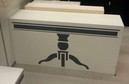
\includegraphics[width=0.3\textwidth]{bar}
				\end{figure}			
			
			\item Cabinet
					\begin{figure}[H]
						\centering
						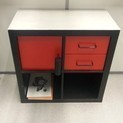
\includegraphics[width=0.25\textwidth]{cabinet}
					\end{figure}	
			
			\item Dinner table
				\begin{figure}[H]
					\centering
					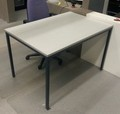
\includegraphics[width=0.25\textwidth]{dinnertable}
				\end{figure}		
		\end{itemize} 
	\item Amigo flight case. Om AMIGO reis bestendig te maken moeten onderstaande stappen gevolgd worden:
		\begin{itemize}
		\item Home alle onderdelen van AMIGO en zet de robot uit.
		\item Doe de kappen over de batterijen van AMIGO indien dit nog niet het geval is.
		\item Open the flight case door aan de sluitingen aan de zijkant te draaien.
		\item Til \textbf{voorzichtig} de bovenste helft van de onderste helft van de casing en leg alle onderdelen die in de casing zitten voorlopig even aan de kant.
		\item Open de voorkant van de onderste helft van de casing, wederom door aan de sluitingen te draaien.
		\item Leg zo veel mogelijk batterijen in de lege ruimte aan de onderkant van de casing.
		\begin{figure}[H]
			\centering
			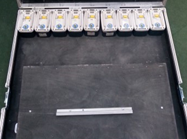
\includegraphics[scale=0.7]{batteries}
		\end{figure}
		\item Draai het dopje in the loopplank los en klap de loopplank uit. \textbf{Let op!} Leg het dopje even weg maar vergeet niet waar ze liggen natuurlijk!
		\item Rijd AMIGO handmatig de loopplank op en til hem op de juiste plek.
		\item Klem de spindel van AMIGO vast aan de casing (deze klem zit op 'buik' hoogte).
		\begin{figure}[H]
			\centering
			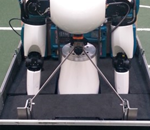
\includegraphics[scale = 0.8]{klem}
		\end{figure}
		\item Klap de loopplank weer in en draai het dopje weer vast.
		\item Draai de microfoon (op het 'hoofd' van AMIGO) zodat deze in de zelfde richting staat als de kinect (de 'ogen'). Gebruik daarna de beschermende materialen in de vorm van een holle cylinder om de camera en de microfoon in te pakken.
		\item Schuif de blokkige beschermende materialen tussen de batterij kappen en de casing. \textbf{Tip:} De twee blokjes zijn niet even groot dus wissel de blokjes om als ze niet goed passen.
		\item Zet de achterkant van AMIGO vast door de houten blokjes vast te draaien met de bijbehorende schroeven.
		\item Schuif de foam blokken \textbf{voorzichtig} op de juiste plekken in de casing. \textbf{Let op!} Zorg ervoor dat de handen van AMIGO niet beschadigen of gedraaid worden.
		\item Doe de onderkant van de casing weer dicht door aan de sluitingen te draaien.
		\item Draai de dopjes uit de planken met de batterij opladers er op. 
		Til deze planken \textbf{voorzichtig} in de casing en draai de dopjes goed aan de casing. 

		\begin{figure}[H]
			\centering
			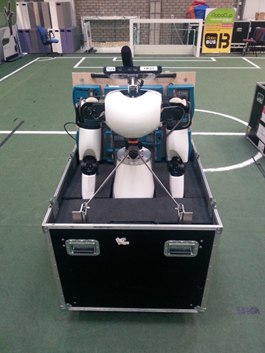
\includegraphics[scale=0.7]{amigo2}
		\end{figure}
		\item Zet de top van de casing \textbf{HEEL VOORZICHTIG} weer terug op de onderkant en draai de sluitingen vast.
		\end{itemize}

\end{itemize}
\end{document}